\subsection{Fouriersynthese}

\begin{figure}[h!]
	\centering
	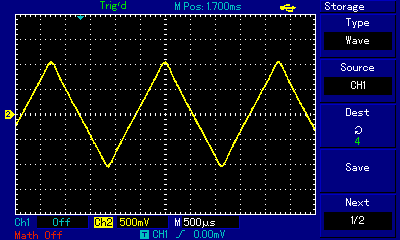
\includegraphics[width=0.95\textwidth]{Synthese_Dreieck.png}
	\caption{Ann�herung an ein Dreiecksignal}
	\label{Synthese_Dreieck}
\end{figure}


\begin{figure}[h!]
	\centering
	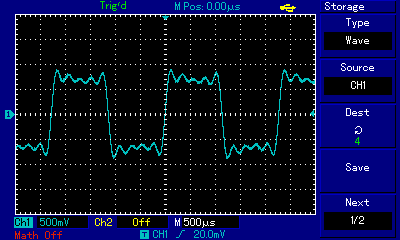
\includegraphics[width=0.95\textwidth]{Synthese_Rechteck.png}
	\caption{Ann�herung an ein Rechtecksignal}
	\label{Synthese_Rechteck}
\end{figure}


\begin{figure}[h!]
	\centering
	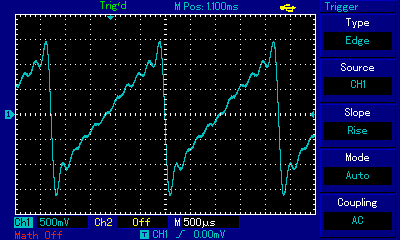
\includegraphics[width=0.95\textwidth]{Synthese_Saegezahn.png}
	\caption{Ann�herung an ein S�gezahnsignal}
	\label{Synthese_Rechteck}
\end{figure}

\clearpage
\subsection{Fourieranalyse}
Die Abweichung der gemessenen und abgelesenen Werte $a_\text{g}$ von den berechneten Werten $a_\text{b}$ wird hier wie folgt berechnet
\begin{equation}
\Delta a = \frac{1}{N-2} \sqrt{ \sum_{i=2}^{N} (a_\text{g} - a_\text{b})^2 } \ .
\end{equation}
Es ist wichtig, bei dem zweiten Wert zu beginnen, da der erste keine Abweichung haben kann. Deswegen wir auch durch $N-2$ geteilt, statt durch $N-1$.

\begin{figure}[h!]
	\centering
	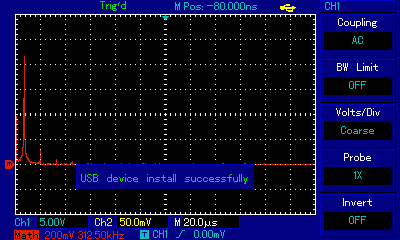
\includegraphics[width=0.95\textwidth]{Dreieck.png}
	\caption{Frequenzspektrum Dreiecksignal}
	\label{Synthese_Dreieck}
\end{figure}


\begin{figure}[h!]
	\centering
	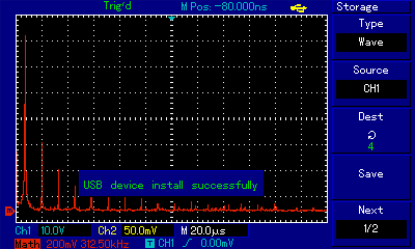
\includegraphics[width=0.95\textwidth]{Rechteck.png}
	\caption{Frequenzspektrum Rechtecksignal}
	\label{Synthese_Rechteck}
\end{figure}


\begin{figure}[h!]
	\centering
	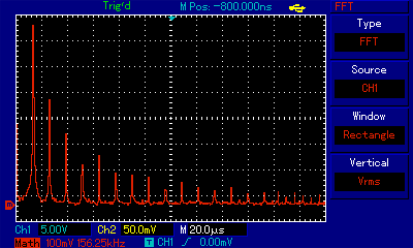
\includegraphics[width=0.95\textwidth]{Saegezahn.png}
	\caption{Frequenzspektrum S�gezahnsignal}
	\label{Synthese_Rechteck}
\end{figure}


\begin{figure}[h!]
	\centering
	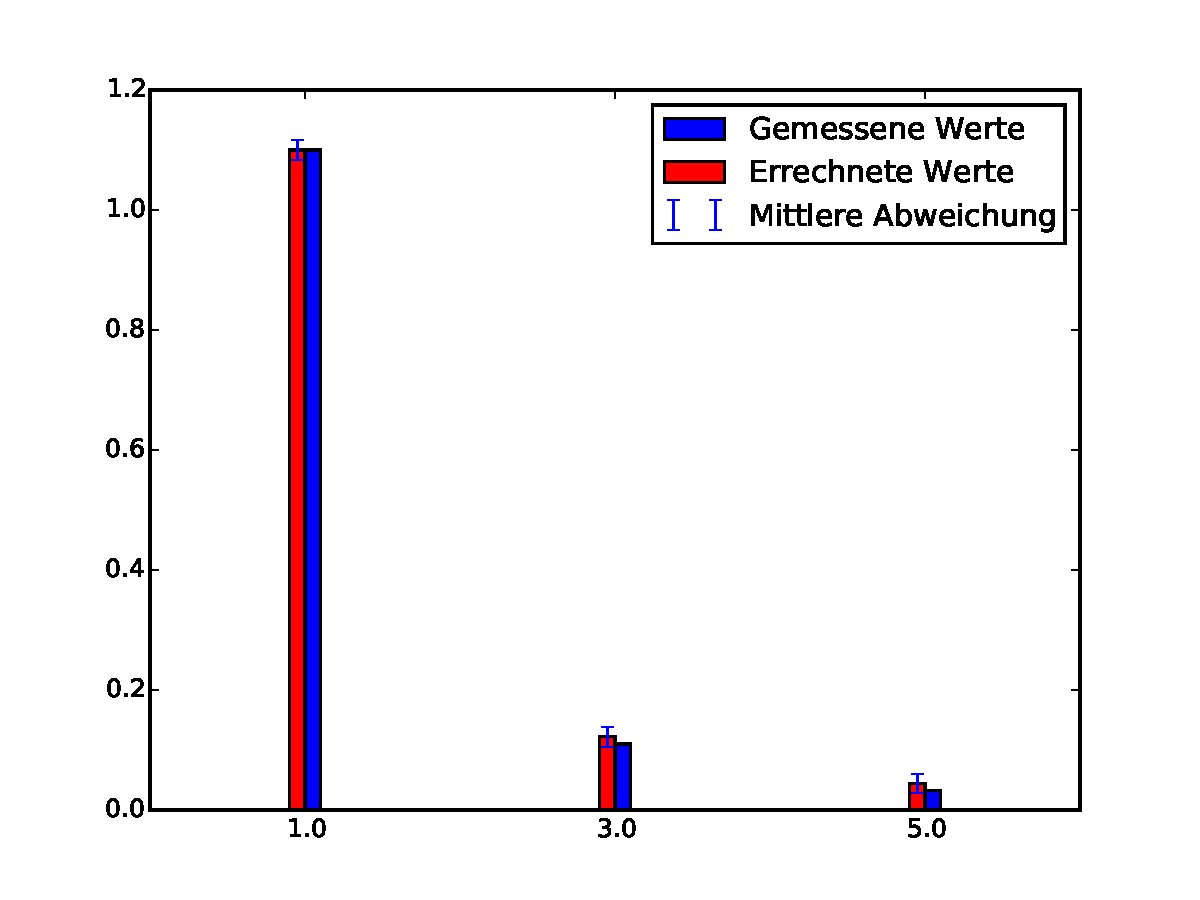
\includegraphics[width=0.95\textwidth]{Dreieck_Fourier.pdf}
	\caption{Frequenzspektrum Dreiecksignal}
	\label{Synthese_Dreieck}
\end{figure}


\begin{figure}[h!]
	\centering
	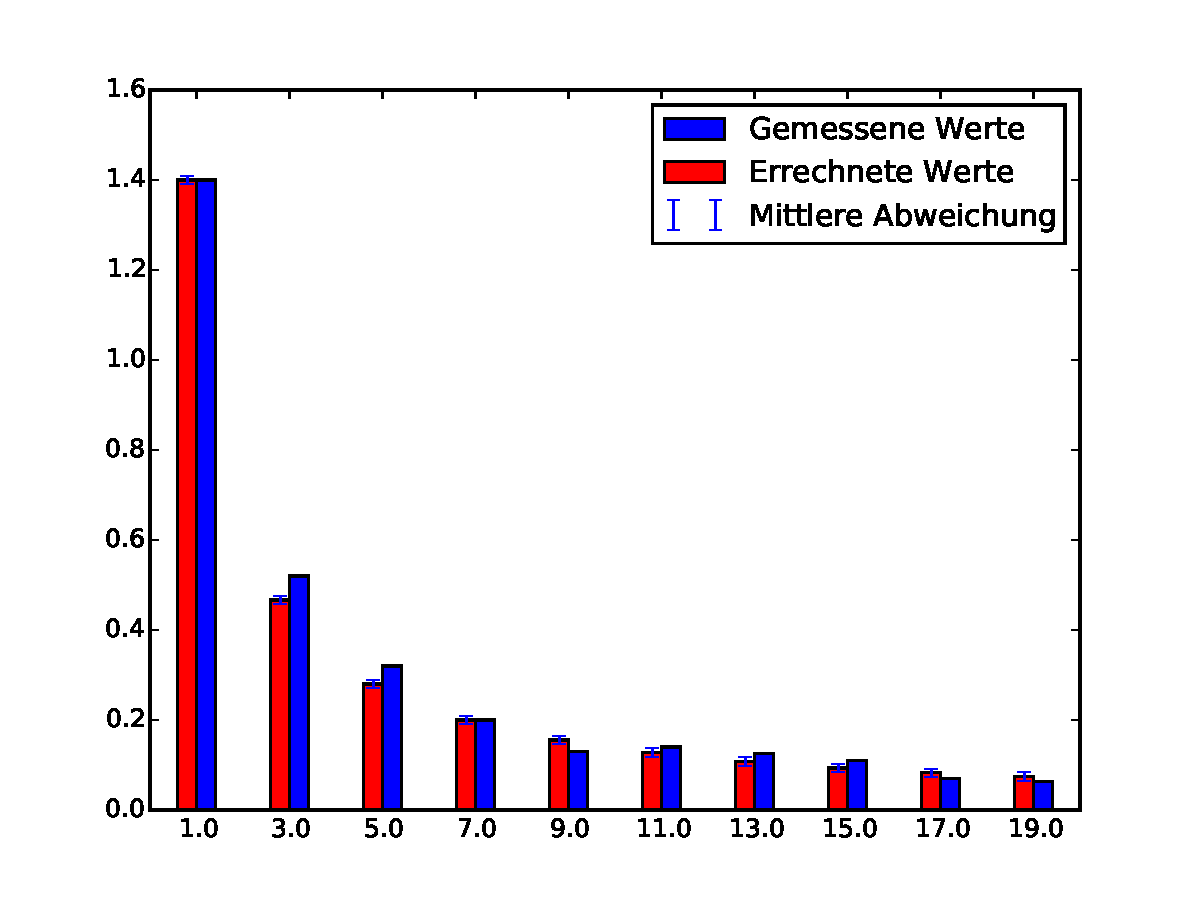
\includegraphics[width=0.95\textwidth]{Rechteck_Fourier.pdf}
	\caption{Frequenzspektrum Rechtecksignal}
	\label{Synthese_Rechteck}
\end{figure}


\begin{figure}[h!]
	\centering
	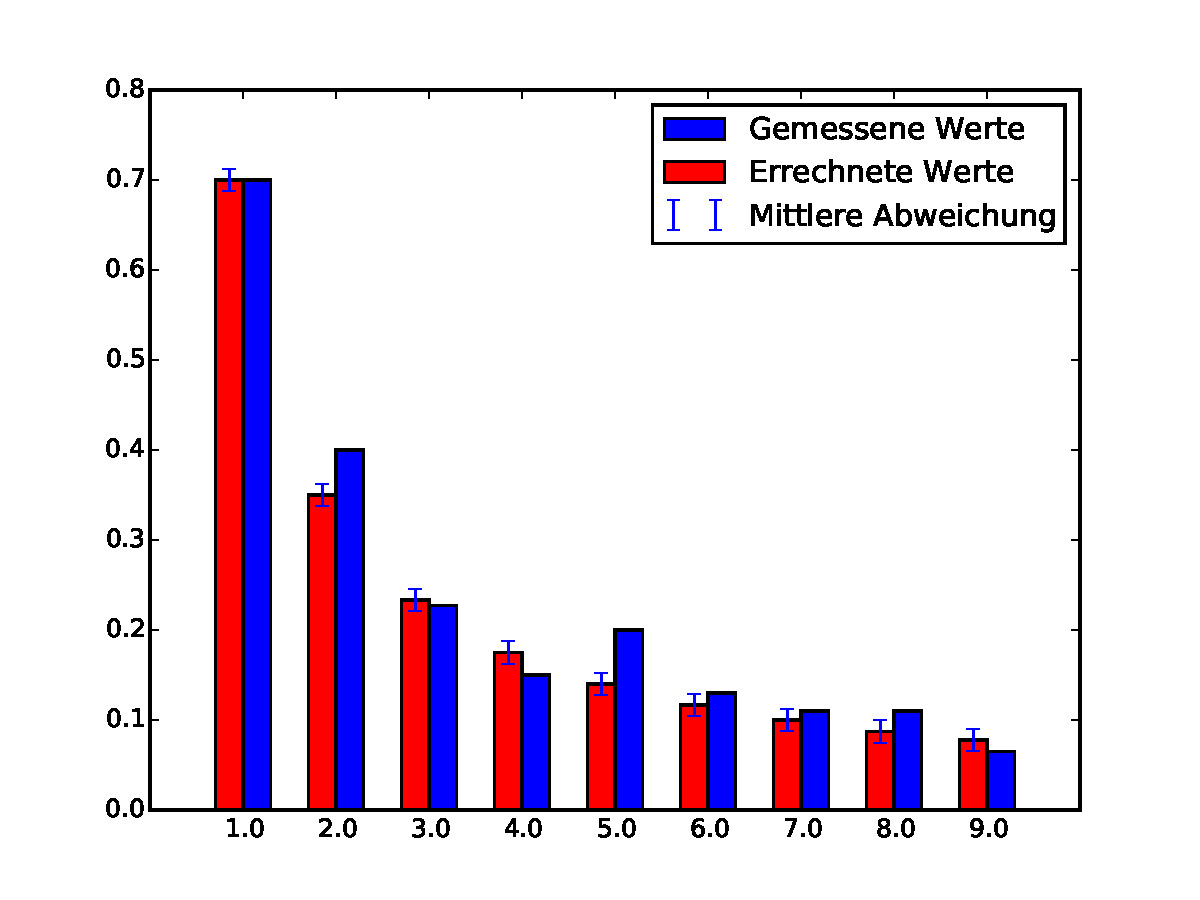
\includegraphics[width=0.95\textwidth]{Saegezahn_Fourier.pdf}
	\caption{Frequenzspektrum S�gezahnsignal}
	\label{Synthese}
\end{figure}
